\documentclass{article}

\usepackage{Sweave}
\begin{document}
\Sconcordance{concordance:DenverPoliceStops.tex:DenverPoliceStops.Rnw:%
1 2 1 1 0 14 1 1 3 8 0 1 2 2 1 1 4 12 0 1 2 2 1 1 4 9 0 1 2 2 1 1 3 9 0 %
1 2 2 1 1 12 1 2 3 1 1 11 1 2 3 1 1 6 1 2 1 1}


\title{Hello Sweave}
\author{cyorir}
\date{September 22, 2018}

\maketitle

The purpose of this article is to serve as an example of a Sweave document. R will be used to examine a dataset from the Denver Open Data Catalog, containing data on Denver Police stops of pedestrians and vehicles. This dataset may be found at \\

https://www.denvergov.org/opendata/dataset/city-and-county-of-denver-police-pedestrian-stops-and-vehicle-stops \\

The dataset contains 14 columns: \\

\begin{Schunk}
\begin{Soutput}
 [1] "MASTER_INCIDENT_NUMBER" "PRIORITY_DESCRIPTION"   "PROBLEM"               
 [4] "ADDRESS"                "CALL_CLASS"             "TIME_PHONEPICKUP"      
 [7] "CALL_DISPOSITION"       "GEO_X"                  "GEO_Y"                 
[10] "GEO_LON"                "GEO_LAT"                "DISTRICT_ID"           
[13] "PRECINCT_ID"            "NEIGHBORHOOD_NAME"     
\end{Soutput}
\end{Schunk}

It is a fair bit of information to take in. Not all of the columns are necessary for this analysis, so only data for columns of interest will be kept. Here is the structure of the reduced dataset: \\

\begin{Schunk}
\begin{Soutput}
'data.frame':	726779 obs. of  8 variables:
 $ PROBLEM          : Factor w/ 2 levels "Subject Stop",....
 $ ADDRESS          : Factor w/ 97823 levels " 11th St / "..
 $ CALL_CLASS       : int  2 2 2 2 2 2 2 2 2 2 ...
 $ TIME_PHONEPICKUP : Factor w/ 720074 levels "2010-12-31"..
 $ CALL_DISPOSITION : Factor w/ 204 levels "1 - Alarm RP "..
 $ GEO_LON          : num  -105 -105 -105 -105 -105 ...
 $ GEO_LAT          : num  39.6 39.6 39.6 39.6 39.6 ...
 $ NEIGHBORHOOD_NAME: Factor w/ 79 levels "Athmar Park",....
\end{Soutput}
\end{Schunk}

Here are the most common addresses for pedestrian stops:\\

\begin{Schunk}
\begin{Soutput}
        16th St / Champa St        1566 N Washington St 
                        580                         651 
     1625 S University Blvd E Colfax Ave / N Downing St 
                        666                         809 
         1499 N BROADWAY ST          1499 N Broadway St 
                       1102                        2240 
\end{Soutput}
\end{Schunk}

Here are the most common addresses for vehicle stops:\\

\begin{Schunk}
\begin{Soutput}
   E 35th Ave / N Syracuse St    W Colfax Ave / N Stuart St 
                         1624                          1757 
 W Colfax Ave / N Tennyson St       I25 Hwy_nb / I70 Hwy_eb 
                         1826                          2316 
W Colfax Ave / N Federal Blvd  Park Ave W / N Globeville Rd 
                         2481                          2781 
\end{Soutput}
\end{Schunk}

Here the density of subject stops is mapped:\\

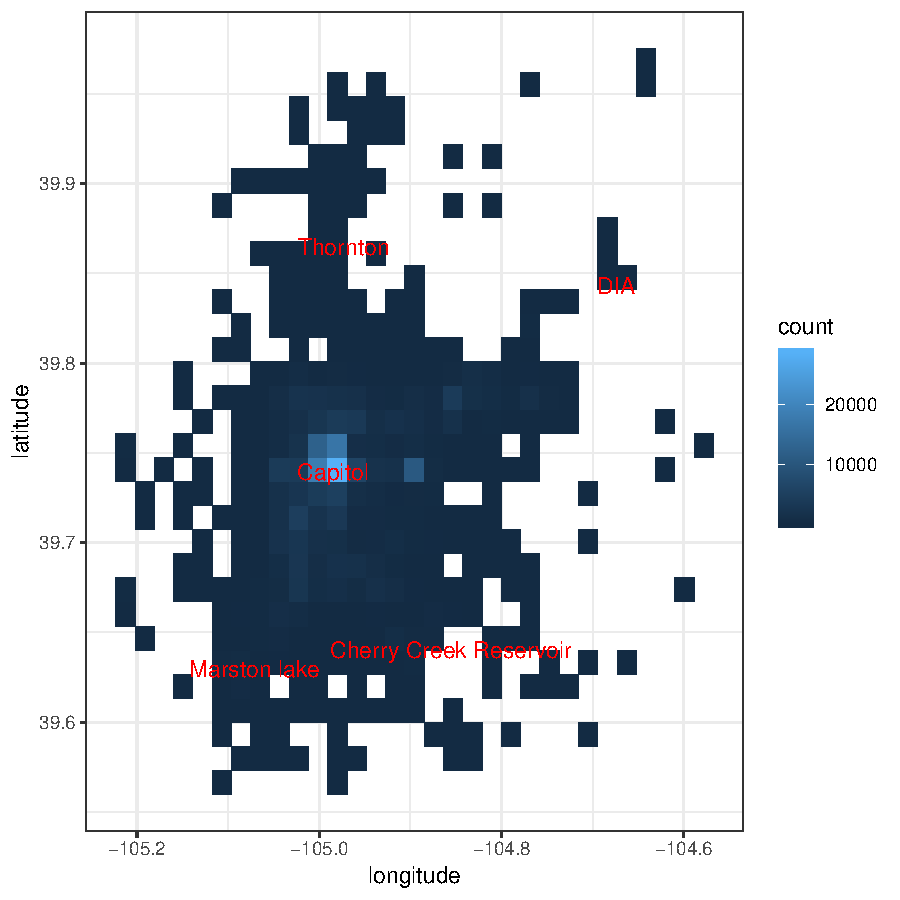
\includegraphics{DenverPoliceStops-005}

\newpage
Here the density of vehicle stops is mapped:\\

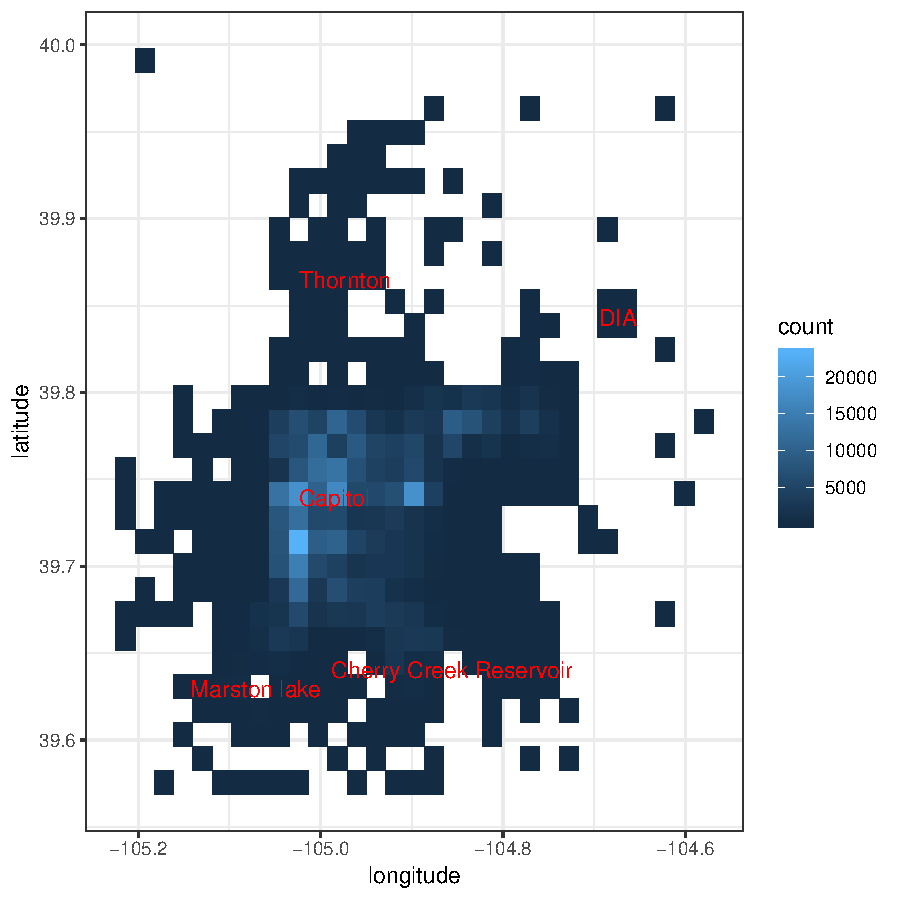
\includegraphics{DenverPoliceStops-006}

\newpage
We can view the number of stops over time:\\

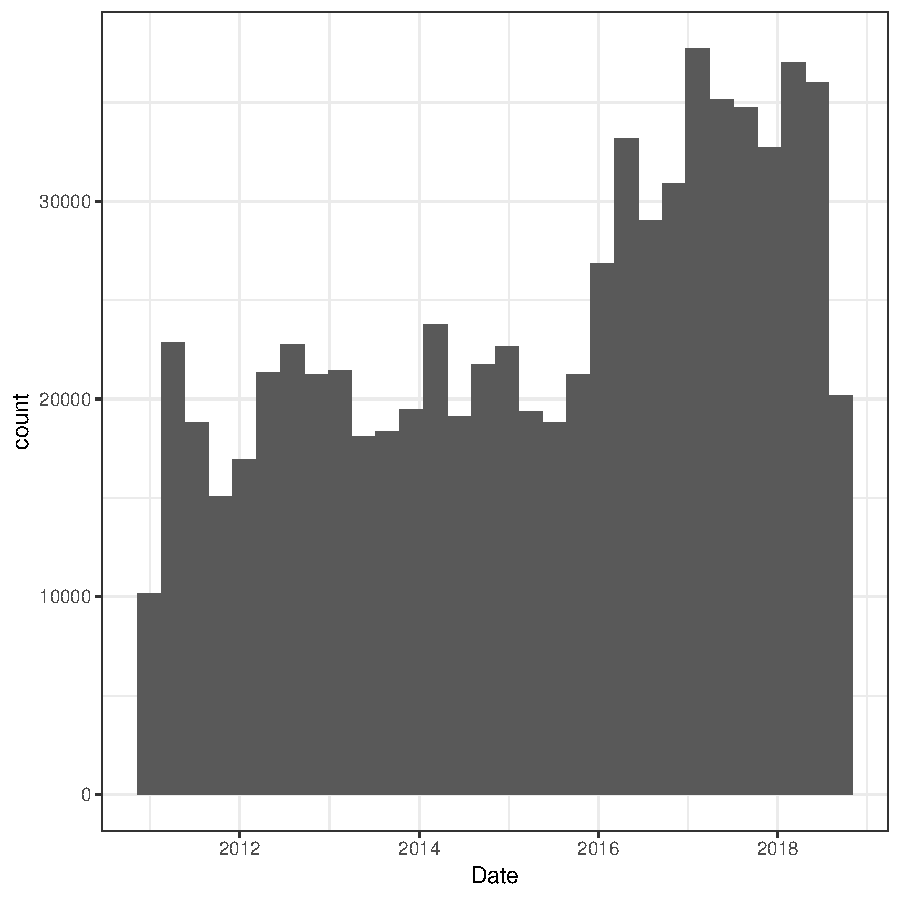
\includegraphics{DenverPoliceStops-007}

\end{document}
